\documentclass{article}\usepackage[]{graphicx}\usepackage[]{xcolor}
% maxwidth is the original width if it is less than linewidth
% otherwise use linewidth (to make sure the graphics do not exceed the margin)
\makeatletter
\def\maxwidth{ %
  \ifdim\Gin@nat@width>\linewidth
    \linewidth
  \else
    \Gin@nat@width
  \fi
}
\makeatother

\definecolor{fgcolor}{rgb}{0.345, 0.345, 0.345}
\newcommand{\hlnum}[1]{\textcolor[rgb]{0.686,0.059,0.569}{#1}}%
\newcommand{\hlsng}[1]{\textcolor[rgb]{0.192,0.494,0.8}{#1}}%
\newcommand{\hlcom}[1]{\textcolor[rgb]{0.678,0.584,0.686}{\textit{#1}}}%
\newcommand{\hlopt}[1]{\textcolor[rgb]{0,0,0}{#1}}%
\newcommand{\hldef}[1]{\textcolor[rgb]{0.345,0.345,0.345}{#1}}%
\newcommand{\hlkwa}[1]{\textcolor[rgb]{0.161,0.373,0.58}{\textbf{#1}}}%
\newcommand{\hlkwb}[1]{\textcolor[rgb]{0.69,0.353,0.396}{#1}}%
\newcommand{\hlkwc}[1]{\textcolor[rgb]{0.333,0.667,0.333}{#1}}%
\newcommand{\hlkwd}[1]{\textcolor[rgb]{0.737,0.353,0.396}{\textbf{#1}}}%
\let\hlipl\hlkwb

\usepackage{framed}
\makeatletter
\newenvironment{kframe}{%
 \def\at@end@of@kframe{}%
 \ifinner\ifhmode%
  \def\at@end@of@kframe{\end{minipage}}%
  \begin{minipage}{\columnwidth}%
 \fi\fi%
 \def\FrameCommand##1{\hskip\@totalleftmargin \hskip-\fboxsep
 \colorbox{shadecolor}{##1}\hskip-\fboxsep
     % There is no \\@totalrightmargin, so:
     \hskip-\linewidth \hskip-\@totalleftmargin \hskip\columnwidth}%
 \MakeFramed {\advance\hsize-\width
   \@totalleftmargin\z@ \linewidth\hsize
   \@setminipage}}%
 {\par\unskip\endMakeFramed%
 \at@end@of@kframe}
\makeatother

\definecolor{shadecolor}{rgb}{.97, .97, .97}
\definecolor{messagecolor}{rgb}{0, 0, 0}
\definecolor{warningcolor}{rgb}{1, 0, 1}
\definecolor{errorcolor}{rgb}{1, 0, 0}
\newenvironment{knitrout}{}{} % an empty environment to be redefined in TeX

\usepackage{alltt}
\usepackage{amsmath} %This allows me to use the align functionality.
                     %If you find yourself trying to replicate
                     %something you found online, ensure you're
                     %loading the necessary packages!
\usepackage{amsfonts}%Math font
\usepackage{graphicx}%For including graphics
\usepackage{hyperref}%For Hyperlinks
\usepackage[shortlabels]{enumitem}% For enumerated lists with labels specified
                                  % We had to run tlmgr_install("enumitem") in R
\hypersetup{colorlinks = true,citecolor=black} %set citations to have black (not green) color
\usepackage{natbib}        %For the bibliography
\setlength{\bibsep}{0pt plus 0.3ex}
\bibliographystyle{apalike}%For the bibliography
\usepackage[margin=0.50in]{geometry}
\usepackage{float}
\usepackage{multicol}
%fix for figures
\usepackage{caption}
\newenvironment{Figure}
  {\par\medskip\noindent\minipage{\linewidth}}
  {\endminipage\par\medskip}
\IfFileExists{upquote.sty}{\usepackage{upquote}}{}
\begin{document}

\vspace{-1in}
\title{Lab 3 -- MATH 240 -- Computational Statistics}

\author{
  Charles Hooey \\
  Student at Colgate University  \\
  Mathematical Economics Major  \\
  {\tt chooey@colgate.edu}
}

\date{}

\maketitle

\begin{multicols}{2}
\begin{abstract}
This laboratory assignment involved the use of R to extract song data from three different bands in order to determine which band contributed most to a specific track. The song data was first sourced in the first part of the lab, cleaned within the second part, and finally summarized within the third part in order to come to a final conclusion that the band Manchester Orchestra had contributed most to the song "Allentown".
\end{abstract}

\noindent \textbf{Keywords:} For Loops; Packages; Lists; Data Frames

\section{Introduction}
This labratory assignment involves the examination of data extracted from songs using Essentia \citep{essentia} in order to determine the degree of contributions by each author made to a song that had been collaborated on by three different bands. Within the first part of this assignment, we seeked to use R in order to replicate a command line that would pull the Essentia data for an individual song for all songs within a specific directory. After sourcing this data, we cleaned and combined it with two other data sources during week two of the assignment. For our third and final week of this assignment, we attempted to make an inference of which band had contributed the most to the song "Allentown" which involved the comparison of Essentia and LIWC features from "Allentown" and other songs released by each of the bands.
\section{Methods}
 As mentioned above, part one of this assignment involves the creation of a batch file in order to process every single song within our music directory through Essentia by generating command prompts that would run the Essentia command for each song, along with each song's file location, and json file format. To complete this task, we made frequent use of the \texttt{stringr} package for \texttt{R} \citep{stringr}, which would assist us in breaking up the locations of each song file into a vector containing the artist, album, track of the song. This vector was established within two seperate loops, one which would sort through all albums and another that would create a new command line for each new song iterated through, and following such each song would have their Essentia command, file location, and json formatted file added to an empty vector that would then be written to a \texttt{.txt} file. Our created batch file would run the Essentia extractor command for each song within the MUSIC directory, which makes data collection much more efficient as had we not written this batch file, we would have had to write the Essentia command line for each individual song. 
\subsection{Collecting and Cleaning Data}
Whereas week one involved the initial sourcing of song data by creating a batch file that would create an Essentia command line for all songs within the MUSIC subdirectory, during week two we seeked to pull data from various files provided within the assignment repository that was for a collection of 181 songs, data which will be helpful in summarizing the musical tendencies of each band who had collaborated on the song "Allentown". In order to complete this task, first within task two we use the \texttt{fromJSON()} function from the \texttt{jsonlite} package in \texttt{R} \citep{jsonlite} in order to pull Essentia model for an example track provided within the assignments repository. After pulling Essentia data for this song, we pulled this data for all files within the EssentiaOutput directory, and cleaned our resulting data by averaging data points that had been calculated using numerous data set into singular columns, and then removing the unaltered data from our data set. After compiling our cleaned data set, we combined this data with data sourced from a language analysis tool called LIWC that was also ran for each of the songs within our directory, as well as the data from our Essentia calls using the \texttt{merge()} function to create one aggregate dataframe.
\subsection{Summarizing Data}
Within the final week of the lab assignment, we used the cleaned song data we had previously sourced in order to collect specific statistical measurements for each band. These measurements included ranges that when compared against data from the song "Allentown" would allow us to determine whether or not each band was in range with the song. The results of this comparison are summarized within Figure \ref{songtab}, which provides data for 10 different musical features. Furthermore, I chose to represent my data visually with a bar chart using \href{https://shiny.colgate.edu/apps/Collaboratory-Apps/ggplots/}{Shiny}, as it provided a simple and easy to interpret graph which showed the relative frequency that each band had been in or out of range when compared with Allentown. 

\section{Results}
 After completing part one of this assignment, I was able to successfully create a batch file containing all songs within the MUSIC directory, which for each song included the command prompt to run Essentia, the file's name, as well as the file listed in json format.  Furthermore, task two of this assignment lead me to source specific Essentia model data values for all songs within a specific directory, and further to merge these values of data with their Essentia call data and LIWC data. The cleaned and aggregated dataset that I had created within week two will provide me with a foundation on which I can make statistical inferences that seek to answer my overarching research question through summarizing data that will help us to better understand specific musical tendencies present within the distinct playstyles of each band. Additionally, I had attempted to solve the lab challenge by creating a boxplot which summarized the pitch salience values of all songs except "Allentown" in an attempt to better understand the vocal tendencies of one of the specific bands that had contributed to the previously mentioned collaboration track. While this graph alone did not provide me any signifigant insight toward my research question, it familiarized me with creating boxplots within \texttt{R}. Finally, the statistical measurements recorded within part three of this lab led me to make the conclusion that Manchester Orchestra had contributed the most to the song "Allentown". As seen within figure \ref{plot1}, among the 10 features included within my data sample, Manchester Orchestra was the only band consistently in range with "Allentown".




%%%%%%%%%%%%%%%%%%%%%%%%%%%%%%%%%%%%%%%%%%%%%%%%%%%%%%%%%%%%%%%%%%%%%%%%%%%%%%%%
% Bibliography
%%%%%%%%%%%%%%%%%%%%%%%%%%%%%%%%%%%%%%%%%%%%%%%%%%%%%%%%%%%%%%%%%%%%%%%%%%%%%%%%
\vspace{2em}



\begin{tiny}
\bibliography{lab3bib}
\end{tiny}
\end{multicols}

%%%%%%%%%%%%%%%%%%%%%%%%%%%%%%%%%%%%%%%%%%%%%%%%%%%%%%%%%%%%%%%%%%%%%%%%%%%%%%%%
% Appendix
%%%%%%%%%%%%%%%%%%%%%%%%%%%%%%%%%%%%%%%%%%%%%%%%%%%%%%%%%%%%%%%%%%%%%%%%%%%%%%%%

\section{Appendix}
Below, I have included my figures and plots for this assignment in order to avoid any formatting issues or complicatations:
\begin{figure}
\caption{Summary of Features by Artist} % Caption for the table
\label{songtab}
% latex table generated in R 4.4.2 by xtable 1.8-4 package
% Tue Feb 25 12:20:01 2025
\begin{table}[H]
\centering
\begingroup\tiny
\begin{tabular}{lll}
  \hline
artist & feature & description \\ 
  \hline
All Get Out & spectral\_skewness & Outlying \\ 
  Manchester Orchestra & spectral\_skewness & Within Range \\ 
  The Front Bottoms & spectral\_skewness & Out of Range \\ 
  All Get Out & spectral\_rolloff & Out of Range \\ 
  Manchester Orchestra & spectral\_rolloff & Within Range \\ 
  The Front Bottoms & spectral\_rolloff & Out of Range \\ 
  All Get Out & spectral\_energyband\_middle\_high & Out of Range \\ 
  Manchester Orchestra & spectral\_energyband\_middle\_high & Within Range \\ 
  The Front Bottoms & spectral\_energyband\_middle\_high & Out of Range \\ 
  All Get Out & spectral\_complexity & Out of Range \\ 
  Manchester Orchestra & spectral\_complexity & Within Range \\ 
  The Front Bottoms & spectral\_complexity & Out of Range \\ 
  All Get Out & spectral\_centroid & Out of Range \\ 
  Manchester Orchestra & spectral\_centroid & Within Range \\ 
  The Front Bottoms & spectral\_centroid & Out of Range \\ 
  All Get Out & melbands\_spread & Out of Range \\ 
  Manchester Orchestra & melbands\_spread & Within Range \\ 
  The Front Bottoms & melbands\_spread & Out of Range \\ 
  All Get Out & melbands\_flatness\_db & Out of Range \\ 
  Manchester Orchestra & melbands\_flatness\_db & Within Range \\ 
  The Front Bottoms & melbands\_flatness\_db & Out of Range \\ 
  All Get Out & erbbands\_skewness & Out of Range \\ 
  Manchester Orchestra & erbbands\_skewness & Within Range \\ 
  The Front Bottoms & erbbands\_skewness & Out of Range \\ 
  All Get Out & erbbands\_flatness\_db & Outlying \\ 
  Manchester Orchestra & erbbands\_flatness\_db & Within Range \\ 
  The Front Bottoms & erbbands\_flatness\_db & Out of Range \\ 
  All Get Out & dissonance & Outlying \\ 
  Manchester Orchestra & dissonance & Within Range \\ 
  The Front Bottoms & dissonance & Out of Range \\ 
   \hline
\end{tabular}
\endgroup
\label{song.tab}
\end{table}

\end{figure}
\begin{figure}[H]
\begin{center}
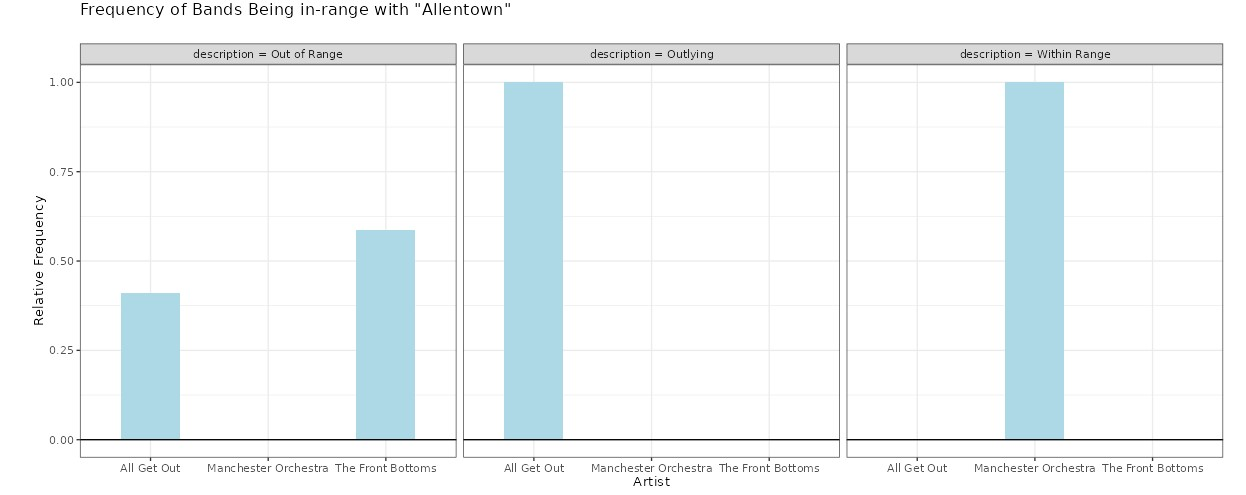
\includegraphics[scale=0.4]{datfigure.jpg}
\caption{Relative Frequency of Each Band Being Within Range of Allentown}
\label{plot1}
\end{center}
\end{figure}
\end{document}
